% หัวข้อย่อย i--iv ของ Top-k (ตัวหนา ไม่มีเลขหัวข้อ)
\providecommand{\topkstep}[1]{\par\medskip\noindent\phantomsection\textbf{#1}\par\nopagebreak\smallskip}

\chapter{\ifproject%
\ifenglish Project Structure and Methodology\else โครงสร้างและขั้นตอนการทำงาน\fi
\else%
\ifenglish Project Structure\else โครงสร้างของโครงงาน\fi
\fi
}

ในบทนี้จะกล่าวถึงภาพรวมของระบบ ชุดข้อมูล การสร้าง Alert และการเตรียมกรณีทดสอบที่ใช้ในการทดลอง
จากนั้นอธิบายการทำงานของ Context Construction Pipeline ทีละขั้นตอน
ตั้งแต่การรับ Alert และ Raw Logs จนถึงการสร้างรายงานการสืบสวน และปิดท้ายด้วยต้นแบบ Web Dashboard
โดยใช้ชุดข้อมูล Account Discovery: Local Account (T1087.001) จาก Splunk Attack Data เป็นตัวอย่างประกอบ

\section{ภาพรวมของระบบ}

ภาพรวมของระบบแสดงดังรูปที่~\ref{fig:overview} แบ่งเป็น 4 ส่วน ได้แก่
\textbf{Input} (Alert และ Raw Logs),
\textbf{Context Construction Pipeline} (Normalize, Event Selection, Representation),
\textbf{Analysis} (RAG และ LLM Analysis) และ \textbf{Output} (Investigation Report)
หมายเลข 1--6 ในรูปคือลำดับขั้นตอนของ Pipeline ซึ่งอธิบายตามลำดับในหัวข้อที่~\ref{sec:step-input}--\ref{sec:step-llm}

\begin{figure}[ht]
\centering
\resizebox{\textwidth}{!}{%
\begin{tikzpicture}[
  node distance=6mm and 7mm,
  box/.style={draw, rounded corners=2pt, fill=white, align=center,
              minimum width=23mm, minimum height=13mm, font=\small},
  arr/.style={-{Latex[length=2.5mm]}, very thick, blue!50!black},
  grp/.style={draw, dashed, rounded corners=8pt, gray, inner sep=3mm},
  stepno/.style={circle, fill=blue!50!black, text=white, font=\scriptsize\bfseries,
               inner sep=0pt, minimum size=4mm}]
  \node[box] (alert) {Alert/EDR\\[-1pt]{\scriptsize ตรวจพบความผิดปกติ}};
  \node[box, below=of alert, label={[stepno]north west:1}] (raw) {Raw Log\\[-1pt]{\scriptsize ไฟล์ Logs}};
  \node[box, right=12mm of raw, label={[stepno]north west:2}] (norm) {Normalize\\[-1pt]{\scriptsize Field ร่วม (CIM)}};
  \node[box, right=of norm, label={[stepno]north west:3}] (sel) {Event Selection\\[-1pt]{\scriptsize คัด Event สำคัญ}};
  \node[box, right=of sel, label={[stepno]north west:4}] (rep) {Representation\\[-1pt]{\scriptsize JSON / TOON}};
  \node[box, right=12mm of rep, label={[stepno]north west:6}] (llm) {LLM Analysis\\[-1pt]{\scriptsize ระบุ Technique}};
  \node[box, above=of llm, label={[stepno]north west:5}] (rag) {RAG\\[-1pt]{\scriptsize ดึง Top-$k$ MITRE}};
  \node[box, right=12mm of llm] (out) {Output\\[-1pt]{\scriptsize Report}};
  \draw[arr] (alert) -- (raw);
  \draw[arr] (raw) -- (norm);
  \draw[arr] (norm) -- (sel);
  \draw[arr] (sel) -- (rep);
  \draw[arr] (rep) -- (llm);
  \draw[arr] (rep.east) ++(4mm,0) |- (rag.west);
  \draw[arr] (rag) -- (llm);
  \draw[arr] (llm) -- (out);
  \begin{scope}[on background layer]
    \node[grp, fit=(alert)(raw), label={[gray]above:Input}] {};
    \node[grp, fit=(norm)(sel)(rep), label={[gray]above:Context Construction Pipeline}] {};
    \node[grp, fit=(rag)(llm), label={[gray]above:Analysis}] {};
    \node[grp, fit=(out), label={[gray]above:Output}] {};
  \end{scope}
\end{tikzpicture}}
\caption{ภาพรวมของระบบและ Context Construction Pipeline (หมายเลข 1--6 คือลำดับขั้นตอนในหัวข้อที่~\ref{sec:pipeline})}
\label{fig:overview}
\end{figure}

หลักการสำคัญของระบบคือ \textbf{ระบบไม่ได้ทำหน้าที่ตรวจจับภัยคุกคามแทน SIEM/EDR}
Alert ที่ระบบเดิมตรวจพบเป็นเพียงจุดเริ่มต้นการสืบสวน (Input ที่รับเข้ามา)
หน้าที่ของ Pipeline คือขยายข้อมูลรอบจุดเริ่มต้นนั้นให้เป็น Investigation Context
ที่ LLM สามารถวิเคราะห์ได้อย่างมีหลักฐาน
การจัดระเบียบข้อมูลก่อนส่งให้ LLM ช่วยลด Noise และทำให้ LLM โฟกัสข้อมูลที่สำคัญได้ดีกว่าการส่ง Raw Logs โดยตรง
Input และ Output ของแต่ละขั้นตอนสรุปได้ดังตารางที่~\ref{tab:pipeline-io}

\begin{table}[ht]
  \centering
  \caption{Input และ Output ของแต่ละขั้นตอนใน Pipeline}
  \label{tab:pipeline-io}
  \small
  \begin{tabular}{|L{0.27\textwidth}|L{0.30\textwidth}|L{0.33\textwidth}|}
    \hline
    \textbf{ขั้นตอน} & \textbf{Input} & \textbf{Output} \\ \hline
    1. รับ Alert และ Raw Logs & ไฟล์ Raw Logs + Alert (Anchor)  & Events ของกรณีทดสอบ (เรียงตามเวลา) \\ \hline
    2. Normalize      & Windows/Linux Raw Logs               & JSON ตามโครงสร้าง Field ร่วม \\ \hline
    3. Event Selection & JSON Logs + Alert                   & Selected JSON Logs \\ \hline
    4. Representation & Selected JSON Logs                   & Representation Log \\ \hline
    5. RAG            & Query จาก Representation Log         & Top-$k$ Techniques (Context) \\ \hline
    6. LLM Analysis   & Context + Representation Log         & Attack Technique พร้อมหลักฐาน \\ \hline
    \phantom{6. }Output & ผลการวิเคราะห์ของ LLM                 & Investigation Report \\ \hline
  \end{tabular}
\end{table}

\section{ชุดข้อมูล}
\label{sec:dataset}

โครงงานไม่ได้จำลองการโจมตีหรือเก็บ Logs ขึ้นเอง แต่ใช้ชุดข้อมูลสาธารณะที่มีผู้บันทึกไว้แล้ว 2 แหล่ง
คือ Splunk Attack Data~\cite{splunk-attack-data} และ OTRF Security-Datasets~\cite{otrf-security-datasets}
ทุกชุดข้อมูลที่ใช้ยึดหลัก \textbf{1 Scenario = 1 เทคนิค} ตามนิยามในหัวข้อที่~\ref{sec:scenario-def}
กล่าวคือ Logs หนึ่งชุดบันทึกการโจมตีเพียงเทคนิคเดียว และเทคนิคนั้นเป็นเฉลยของ Scenario

\subsection{การคัดเลือกเทคนิค}
ก่อนอธิบายเกณฑ์ ขอนิยามคำที่ใช้ในหัวข้อนี้ดังนี้
\begin{itemize}
  \item \textbf{Windows Atomic (OTRF)} -- ชุดข้อมูลหมวด Atomic ของ OTRF ที่บันทึกจากเครื่อง Windows
        โดย 1 ชุดจำลองการโจมตีเพียง 1 เทคนิค ตรงกับหลัก 1 Scenario = 1 เทคนิค
        ส่วน OTRF หมวด Compound จำลองทั้ง Campaign ที่มีหลายเทคนิคต่อเนื่องกัน (เช่น การจำลองกลุ่ม APT29)
        ซึ่งไม่ตรงกับหลักดังกล่าว โครงงานจึง\textbf{ไม่ใช้}ชุดข้อมูลหมวด Compound
  \item \textbf{Atomic Red Team (ART)}~\cite{atomic-red-team} -- คลังชุดทดสอบการโจมตีแบบโอเพนซอร์สของ Red Canary
        แยกตามเทคนิค ATT\&CK โดยแต่ละชุดทดสอบเขียนคำสั่งที่ใช้โจมตีไว้ชัดเจนในไฟล์ YAML
        และรันผ่านคำสั่ง PowerShell \texttt{Invoke-AtomicTest}
        (คำว่า Atomic ในชื่อเครื่องมือหมายถึงชุดทดสอบขนาดเล็กที่ทดสอบทีละเทคนิค)
  \item \textbf{ชุดข้อมูล ART ของ Splunk} -- ชุดข้อมูลในโฟลเดอร์ \texttt{atomic\_red\_team} ของ Splunk Attack Data
        ซึ่งทีมของ Splunk เป็นผู้รัน Atomic Red Team ใน Lab ที่สร้างด้วย attack\_range และบันทึก Logs ไว้
        โดยแต่ละโฟลเดอร์เป็นของเทคนิคเดียว
\end{itemize}

เหตุผลที่เลือกเฉพาะชุดข้อมูล ART ของ Splunk เป็น Development Set คือ
ชุดข้อมูลแบบนี้รู้คำสั่งโจมตีล่วงหน้า และใน Logs มีร่องรอยของคำสั่ง \texttt{Invoke-AtomicTest}
หรือไฟล์จากโฟลเดอร์ \texttt{AtomicRedTeam} เป็นจุดเริ่มต้นของการโจมตี
จึงไล่ตาม Process Tree เพื่อระบุ Event ที่เป็นการโจมตี (Ground Truth ระดับ Event) ได้อัตโนมัติ
ส่วนชุดข้อมูลในโฟลเดอร์อื่น เช่น \texttt{snapattack} หรือชุดที่จำลองด้วยมือ ไม่มีร่องรอยดังกล่าว
ต้องระบุ Event ที่เป็นการโจมตีด้วยมือทั้งหมด ซึ่งใช้เวลามากและตรวจสอบซ้ำได้ยาก
นอกจากนี้ ART ยังเป็นเครื่องมือมาตรฐานที่ใช้แพร่หลาย แต่ละชุดทดสอบตรงกับเทคนิคเดียว และทำซ้ำได้

เทคนิคที่ใช้ทดลองถูกคัดเลือกด้วยเกณฑ์ที่กำหนดไว้ล่วงหน้า ไม่ได้เลือกด้วยมือ
ดังตารางที่~\ref{tab:technique-funnel} โดยขั้นที่ 0--1 นับเป็นจำนวนไฟล์หรือชุดข้อมูล
ขั้นที่ 2--3 นับเป็นจำนวนเทคนิค และขั้นที่ 4 นับเป็นจำนวนไฟล์และชุดข้อมูลที่ใช้ทดลองจริง
ตัวเลขทั้งหมดนับจาก Repository ที่ระบุ Commit ไว้ในตารางที่~\ref{tab:snapshot}

\begin{table}[ht]
  \centering
  \caption{ขั้นตอนการคัดเลือกเทคนิคสำหรับการทดลอง}
  \label{tab:technique-funnel}
  \small
  \begin{tabular}{|c|L{0.25\textwidth}|L{0.33\textwidth}|L{0.25\textwidth}|}
    \hline
    \textbf{ขั้น} & \textbf{เกณฑ์} & \textbf{ผล} & \textbf{เหตุผล} \\ \hline
    0 & Metadata ทั้งหมด &
      Splunk 1,030 ไฟล์ YAML (313 เทคนิค) / OTRF 100 ชุด Windows Atomic & จุดเริ่มต้น \\ \hline
    1 & Windows Sysmon และระบุเทคนิคเดียว &
      Splunk 425 ไฟล์ YAML (193 เทคนิค) / OTRF 97 ชุดที่มี Sysmon Event อย่างน้อย 1 รายการเมื่อเปิดอ่านไฟล์จริง (50 เทคนิค) &
      ต้องมีข้อมูล Sysmon ให้วิเคราะห์ และ Ground Truth เป็นเทคนิคเดียว \\ \hline
    2 & เทคนิคที่มีในทั้งสองแหล่ง & 42 เทคนิค & Development Set และ Test Set ต้องครอบคลุมเทคนิคเดียวกัน \\ \hline
    3 & Splunk มีชุดข้อมูล Atomic Red Team & \textbf{24 เทคนิค} & ระบุ Event สำคัญได้อัตโนมัติเฉพาะชุด ART \\ \hline
    4 & เลือกไฟล์และชุดข้อมูลของ 24 เทคนิค &
      Dev: ไฟล์ Sysmon ของชุด ART \textbf{38 ไฟล์} / Test: OTRF 54 ชุด จำกัดไม่เกิน 3 ชุดต่อเทคนิค เหลือ \textbf{42 ชุด} &
      รายละเอียดในหัวข้อ~\ref{sec:dev-test} \\ \hline
  \end{tabular}
\end{table}

\begin{table}[ht]
  \centering
  \caption{เวอร์ชันของ Repository ที่ใช้ (Snapshot)}
  \label{tab:snapshot}
  \small
  \begin{tabular}{|l|l|l|}
    \hline
    \textbf{Repository} & \textbf{Commit} & \textbf{วันที่} \\ \hline
    splunk/attack\_data & \texttt{f08d681} & 29 ต.ค. 2569 \\ \hline
    OTRF/Security-Datasets & \texttt{d9d40ef} & 20 ก.ย. 2566 (รุ่นล่าสุด) \\ \hline
    splunk/security\_content (ESCU) & \texttt{dcd2560} & 30 ต.ค. 2569 \\ \hline
  \end{tabular}
\end{table}

ชุดข้อมูล T1087.001 ที่ใช้เป็นตัวอย่างตลอดบทนี้ไม่ผ่านเกณฑ์ขั้นที่ 3
เนื่องจาก Splunk ไม่มีชุดข้อมูล Atomic Red Team ของเทคนิคนี้
จึงใช้เป็นกรณีนำร่อง (Pilot) สำหรับตรวจสอบว่า Pipeline ทำงานได้ครบทุกขั้นตอนเท่านั้น

\subsection{Development Set และ Test Set}
\label{sec:dev-test}
\textbf{Development Set} มาจากไฟล์ Sysmon ในชุดข้อมูล ART ของ Splunk ที่ตรงกับ 24 เทคนิค
ซึ่ง Metadata ระบุไว้ 39 ไฟล์ แต่มีไฟล์จริงใน Repository \textbf{38 ไฟล์}
(ไฟล์ \texttt{T1021.002/dns-sysmon.log} ถูกระบุใน Metadata แต่ไม่มีใน Repository)
ใช้สำหรับปรับพารามิเตอร์และ Prompt ของ Pipeline

\textbf{Test Set} ประกอบด้วยชุดข้อมูล OTRF แบบ Windows Atomic จำนวน \textbf{42 ชุด}
คัดจาก 54 ชุดที่ตรงกับ 24 เทคนิคและมีไฟล์ Sysmon ใช้งานได้
แล้วจำกัดไม่เกิน 3 ชุดต่อเทคนิค ด้วยกฎ ``เลือกชุดที่ใช้เครื่องมือต่างกันก่อน ถ้าเท่ากันเลือกชุดที่เก่ากว่า''
จำนวนข้อมูลแยกตามเทคนิคแสดงในตารางที่~\ref{tab:dev-test}

เหตุผลที่ใช้ Splunk เป็น Development Set และ OTRF เป็น Test Set คือ
ชุดข้อมูล Atomic Red Team ของ Splunk ระบุ Event สำคัญได้อัตโนมัติ
ส่วน OTRF มาจาก Lab และเครื่องมือโจมตีที่ต่างกัน (เช่น Empire และ Covenant)
จึงทดสอบได้ว่าค่าที่ปรับบนข้อมูลของ Splunk ใช้กับข้อมูลจากแหล่งอื่นได้หรือไม่
และป้องกันไม่ให้ลักษณะเฉพาะของสภาพแวดล้อมเดียวกันรั่วจาก Development Set ไปยัง Test Set

\begin{table}[htbp]
  \centering
  \caption{จำนวนข้อมูลใน Development Set และ Test Set แยกตามเทคนิค}
  \label{tab:dev-test}
  \small
  \begin{tabular}{|l|L{0.52\textwidth}|c|c|}
    \hline
    \textbf{เทคนิค} & \textbf{ชื่อ} & \textbf{Dev (ไฟล์)} & \textbf{Test (ชุด)} \\ \hline
    T1003.001 & OS Credential Dumping: LSASS Memory & 3 & 3 \\ \hline
    T1003.002 & OS Credential Dumping: Security Account Manager & 1 & 3 \\ \hline
    T1003.003 & OS Credential Dumping: NTDS & 1 & 3 \\ \hline
    T1021.002 & Remote Services: SMB/Windows Admin Shares & 3 & 3 \\ \hline
    T1047 & Windows Management Instrumentation & 1 & 3 \\ \hline
    T1053.005 & Scheduled Task/Job: Scheduled Task & 1 & 3 \\ \hline
    T1059.001 & Command and Scripting Interpreter: PowerShell & 3 & 1 \\ \hline
    T1069.001 & Permission Groups Discovery: Local Groups & 1 & 2 \\ \hline
    T1112 & Modify Registry & 4 & 3 \\ \hline
    T1197 & BITS Jobs & 1 & 1 \\ \hline
    T1218.001 & System Binary Proxy Execution: Compiled HTML File & 2 & 1 \\ \hline
    T1218.002 & System Binary Proxy Execution: Control Panel & 1 & 1 \\ \hline
    T1218.004 & System Binary Proxy Execution: InstallUtil & 2 & 1 \\ \hline
    T1218.005 & System Binary Proxy Execution: Mshta & 2 & 3 \\ \hline
    T1218.010 & System Binary Proxy Execution: Regsvr32 & 1 & 1 \\ \hline
    T1220 & XSL Script Processing & 1 & 1 \\ \hline
    T1222.001 & Windows File and Directory Permissions Modification & 1 & 1 \\ \hline
    T1543.003 & Create or Modify System Process: Windows Service & 2 & 1 \\ \hline
    T1546.003 & Event Triggered Execution: WMI Event Subscription & 1 & 1 \\ \hline
    T1547.001 & Boot or Logon Autostart: Registry Run Keys & 2 & 2 \\ \hline
    T1548.002 & Abuse Elevation Control: Bypass UAC & 1 & 1 \\ \hline
    T1550.002 & Use Alternate Authentication Material: Pass the Hash & 1 & 1 \\ \hline
    T1562.004 & Impair Defenses: Disable or Modify System Firewall & 1 & 1 \\ \hline
    T1574.001 & Hijack Execution Flow: DLL & 1 & 1 \\ \hline
    \multicolumn{2}{|r|}{\textbf{รวม}} & \textbf{38} & \textbf{42} \\ \hline
  \end{tabular}
\end{table}

ชุดข้อมูลใน Test Set บางชุดมีป้ายกำกับเทคนิคที่น่าสงสัย เช่น ชุด Rubeus ASKTGT ที่ระบุเป็น T1003.003
แต่เป็นพฤติกรรมเกี่ยวกับ Kerberos Ticket และชุด MSBuild ที่ระบุเป็น T1047
ซึ่งจะทบทวนก่อนล็อกค่าการทดลอง หากตัดชุดใดออกจะเลือกชุดถัดไปตามกฎเดิม
ทั้งนี้ ชุดข้อมูลใน Test Set ผ่านการตรวจว่ามี Sysmon Event แล้ว
แต่ยังต้องเทียบกับคำสั่งใน Adversary View ตามหัวข้อ~\ref{sec:case-prep} จำนวนกรณีจริงจึงอาจลดลง

หากในอนาคตพบชุดข้อมูลเพิ่มเติม เช่น ชุดข้อมูลใหม่ใน Repository ของ Splunk หรือ OTRF หรือจากแหล่งอื่น
จะพิจารณานำมาใช้โดยผ่านเกณฑ์ชุดเดียวกันในตารางที่~\ref{tab:technique-funnel}
และบันทึก Commit ที่ใช้ใหม่ ทั้งนี้ชุดข้อมูลที่เพิ่มหลังจากล็อกค่าการทดลองแล้ว
จะรายงานเป็นการประเมินเพิ่มเติมแยกจากผลหลัก เพื่อไม่ให้กระทบความเป็นกลางของ Test Set

\subsection{รูปแบบ Logs ดิบ}
แม้ใช้เฉพาะ Windows Sysmon แต่ Logs ดิบยังมี 3 รูปแบบ (ตารางที่~\ref{tab:raw-formats})
ขั้นตอน Normalize จึงจำเป็นต่อการทำให้ขั้นตอนถัดไปทำงานกับข้อมูลทุกแหล่งได้ด้วยตรรกะเดียวกัน
สำหรับ Linux Auditd แม้ Splunk มีชุดข้อมูล 73 ไฟล์ (33 เทคนิค) แต่ OTRF มีชุดข้อมูล Linux แบบ Atomic เพียง 2 ชุด
และไม่ตรงกับเทคนิคใดของ Splunk จึงสร้าง Development Set และ Test Set ข้ามแหล่งไม่ได้
ระบบจึงรองรับ Auditd ในขั้นตอน Normalize แต่ไม่ประเมินความถูกต้อง

\begin{table}[ht]
  \centering
  \caption{รูปแบบ Logs ดิบที่ต้อง Normalize}
  \label{tab:raw-formats}
  \small
  \begin{tabular}{|l|l|l|}
    \hline
    \textbf{แหล่ง} & \textbf{รูปแบบ} & \textbf{จำนวน} \\ \hline
    Splunk & XmlWinEventLog (XML) & Development Set ทั้งหมด \\ \hline
    OTRF & JSON แบบแบน (\texttt{Channel}, \texttt{EventID}) & 104 ไฟล์ \\ \hline
    OTRF & JSON ซ้อนชั้นของ Winlogbeat 6 (\texttt{log\_name}, \texttt{event\_id}) & 2 ไฟล์ \\ \hline
  \end{tabular}
\end{table}

\section{การสร้าง Alert}
\label{sec:alert}

เพื่อให้จุดเริ่มต้นของการสืบสวนใกล้เคียงการใช้งานจริง
แนวทางการสร้าง Alert ของโครงงานคือใช้ Detection Rule ทางการจาก ES Content Update (ESCU)~\cite{splunk-escu}
แทนการกำหนดเงื่อนไขขึ้นเอง ESCU รวม Rule ทั้งหมดไว้ใน App เดียว
และต้องใช้ร่วมกับ App ที่แปลงข้อมูลให้อยู่ในรูปแบบที่ Rule อ่านได้ ดังตารางที่~\ref{tab:splunk-apps}
จาก Rule ที่ใช้งานได้ทั้งหมด 2,078 Rule มี 928 Rule ที่ใช้ Windows Sysmon
แบ่งเป็นประเภท TTP 484 Rule, Anomaly 345 Rule และ Hunting 99 Rule
โครงงานใช้ประเภท TTP และ Anomaly รวม 829 Rule เนื่องจาก Hunting ไม่สร้าง Alert

\begin{table}[ht]
  \centering
  \caption{App ที่ใช้ร่วมกับ Rule ของ ESCU}
  \label{tab:splunk-apps}
  \small
  \begin{tabular}{|l|c|c|}
    \hline
    \textbf{App} & \textbf{Splunkbase ID} & \textbf{เวอร์ชัน} \\ \hline
    Splunk Common Information Model & 1621 & 8.5.0 \\ \hline
    Splunk Add-on for Sysmon & 5709 & 5.0.0 \\ \hline
    Splunk Add-on for Microsoft Windows & 742 & 10.0.1 \\ \hline
    ES Content Update (ESCU) & 3449 & 6.10.0 \\ \hline
  \end{tabular}
\end{table}

แนวทางการสร้าง Alert มีดังนี้
\begin{enumerate}
  \item แปลงชุดข้อมูล OTRF จาก JSON เป็น Sysmon XML
        เนื่องจาก Splunk Add-on for Sysmon อ่านเฉพาะรูปแบบ XmlWinEventLog
  \item นำ Logs เข้าระบบทีละไฟล์ แล้วรัน Rule ทั้ง 829 Rule
        เพื่อให้ทราบว่า Alert แต่ละรายการมาจากไฟล์ใด
  \item ระบุว่า Alert เป็น True Positive หรือ False Positive
        โดย Development Set ตรวจจาก Process Tree ของ Atomic Red Team
        และ Test Set ตรวจจาก Rule ที่คู่กับชุดข้อมูลเทียบกับ Adversary View
\end{enumerate}

การตรวจสอบว่าแต่ละเทคนิคใน Development Set และ Test Set มี Rule ประเภท TTP หรือ Anomaly รองรับหรือไม่
ยังไม่ได้ดำเนินการ และจะตรวจสอบเมื่อรัน Rule กับชุดข้อมูลจริงในระยะถัดไป
เทคนิคที่ไม่มี Rule รองรับจะใช้ Anchor สำรองตามหัวข้อที่~\ref{sec:case-prep}

ในการทดลองหลักจะใช้ Alert ที่เป็น True Positive 1 รายการต่อไฟล์ ส่วน False Positive นับไว้เพื่อรายงานเท่านั้น
การเลือกหรือจัดกลุ่ม Alert เมื่อมีหลายรายการเป็นประเด็นที่จะศึกษาต่อ
ข้อมูลที่ส่งให้ LLM คือ Event ที่ทำให้เกิด Alert โดยตัดชื่อ Rule และป้ายกำกับ ATT\&CK ออก
เพื่อให้ LLM ต้องระบุเทคนิคจากหลักฐานเอง

ในระยะ Project Survey นี้ Pipeline ยังไม่ได้เชื่อมต่อกับ SIEM โดยตรง
Alert ของแต่ละกรณีทดสอบจึงกำหนดเป็น Event ที่ใช้เป็นจุดเริ่มต้น (Anchor) ซึ่งบันทึกไว้ในไฟล์กรณีทดสอบ
(หัวข้อที่~\ref{sec:case-prep}) ส่วนการรับ Alert จาก SIEM โดยตรงจะพัฒนาในระยะถัดไป

\section{การเตรียมกรณีทดสอบ}
\label{sec:case-prep}

ก่อนการทดลอง ชุดข้อมูลทุกชุดผ่านขั้นตอนเตรียมกรณีทดสอบ (Case) ดังนี้
\begin{enumerate}
  \item \textbf{Freeze} -- ระบุ Commit ของทุก Repository และบันทึก Checksum ของทุกไฟล์
  \item \textbf{Normalize} -- แปลง Logs ทั้ง 3 รูปแบบเป็น JSON ตามหัวข้อที่~\ref{sec:step-normalize}
  \item \textbf{Screening} -- ตรวจว่าไฟล์ของทั้งสองแหล่งมี Sysmon Event ที่เกี่ยวข้องกับคำสั่งโจมตี
        (ไม่จำเป็นต้องเป็น EID 1) โดยไฟล์ของ Splunk ตรวจเทียบกับคำสั่งของชุดทดสอบ Atomic Red Team
        ส่วนชุดของ OTRF ตรวจเทียบกับคำสั่งใน Adversary View และทบทวนชุดที่ป้ายกำกับน่าสงสัย
  \item \textbf{สร้าง Alert} -- ตามแนวทางในหัวข้อที่~\ref{sec:alert}
  \item \textbf{สร้างกรณีทดสอบ} -- 1 Alert ที่เป็น True Positive = 1 กรณี
        ไฟล์ที่ไม่มี Alert ใช้ Event ของคำสั่งโจมตี (EID 1 หรือ Event ที่ตรงกับ Adversary View) เป็น Anchor สำรองและติดธงแยกไว้
  \item \textbf{Leak Check} -- ตัดชื่อ Rule ป้ายกำกับ ATT\&CK และข้อความรูปแบบ \texttt{T\#\#\#\#} ออกจากทุก Prompt
\end{enumerate}

\section{การทำงานของ Pipeline}
\label{sec:pipeline}

หัวข้อนี้อธิบายการทำงานของ Context Construction Pipeline ทีละขั้นตอนตามหมายเลข 1--6 ในรูปที่~\ref{fig:overview}
ทุกกรณีทดสอบผ่านขั้นตอนชุดเดียวกัน ต่างกันเฉพาะวิธีหรือรูปแบบที่กำหนดในแต่ละการทดลอง

\subsection{ขั้นตอนที่ 1: การรับ Alert และ Raw Logs}
\label{sec:step-input}

ในระยะ Project Survey นี้ Pipeline ยังไม่ได้ดึงข้อมูลจาก SIEM โดยตรง
แต่รับ Raw Logs เป็นไฟล์จากชุดข้อมูล (\texttt{.xml}, \texttt{.json}, \texttt{.jsonl} หรือ \texttt{.zip} ที่รวมหลายไฟล์)
และรับ Alert จากไฟล์กรณีทดสอบ ซึ่งระบุ Event ที่ใช้เป็น Anchor (หัวข้อที่~\ref{sec:alert})
ระบบอ่าน Logs ทุกไฟล์ของกรณีเดียวกันแล้วรวมเป็นชุด Events เดียวที่เรียงตามเวลา
Output ของขั้นตอนนี้คือ Events ทั้งหมดของกรณีทดสอบพร้อมจำนวน Events ที่จะส่งต่อไปยังขั้นตอน Normalize
สำหรับชุดข้อมูลตัวอย่าง T1087.001 ซึ่งเป็น Windows Sysmon Logs จาก Splunk Attack Data
มีจำนวน 11,090 Events ในช่วงเวลาประมาณ 15 นาที (ขนาดไฟล์ XML ประมาณ 16.8 MB)
ส่วนการเชื่อมต่อกับ SIEM เพื่อรับ Alert และดึง Logs อัตโนมัติเป็นงานที่จะพัฒนาในระยะถัดไป

\subsection{ขั้นตอนที่ 2: Normalize}
\label{sec:step-normalize}

Raw Logs จากแต่ละแหล่งมีรูปแบบต่างกัน เช่น Sysmon ในชุดข้อมูลของ Splunk Attack Data อยู่ในรูป \texttt{XmlWinEventLog}
และ Auditd เป็นข้อความหลาย Record ต่อเหตุการณ์
และชุดข้อมูล OTRF อยู่ในรูป JSON 2 แบบ (ตารางที่~\ref{tab:raw-formats})
ขั้นตอน Normalize จะ Parse Logs แล้วแปลงเป็น JSON ที่มีโครงสร้าง Field ร่วม (Common Field Structure)
ที่อิงแนวคิดของ Splunk CIM~\cite{splunk-cim} คือใช้ชื่อ Field ชุดเดียวกันไม่ว่า Logs จะมาจากแหล่งใด
ตัวอย่าง Field ที่ใช้ เช่น \texttt{EventID}, \texttt{SystemTime}, \texttt{RecordNumber},
\texttt{Channel}, \texttt{Image}, \texttt{CommandLine}, \texttt{ProcessGuid}, \texttt{ParentProcessGuid} และ \texttt{User}
ดังตัวอย่างในรูปที่~\ref{fig:normalize}
ผลลัพธ์ทำให้ขั้นตอนถัดไปทำงานกับ Logs จากทั้ง Windows และ Linux ได้ด้วยตรรกะเดียวกัน

\begin{figure}[ht]
  \centering
  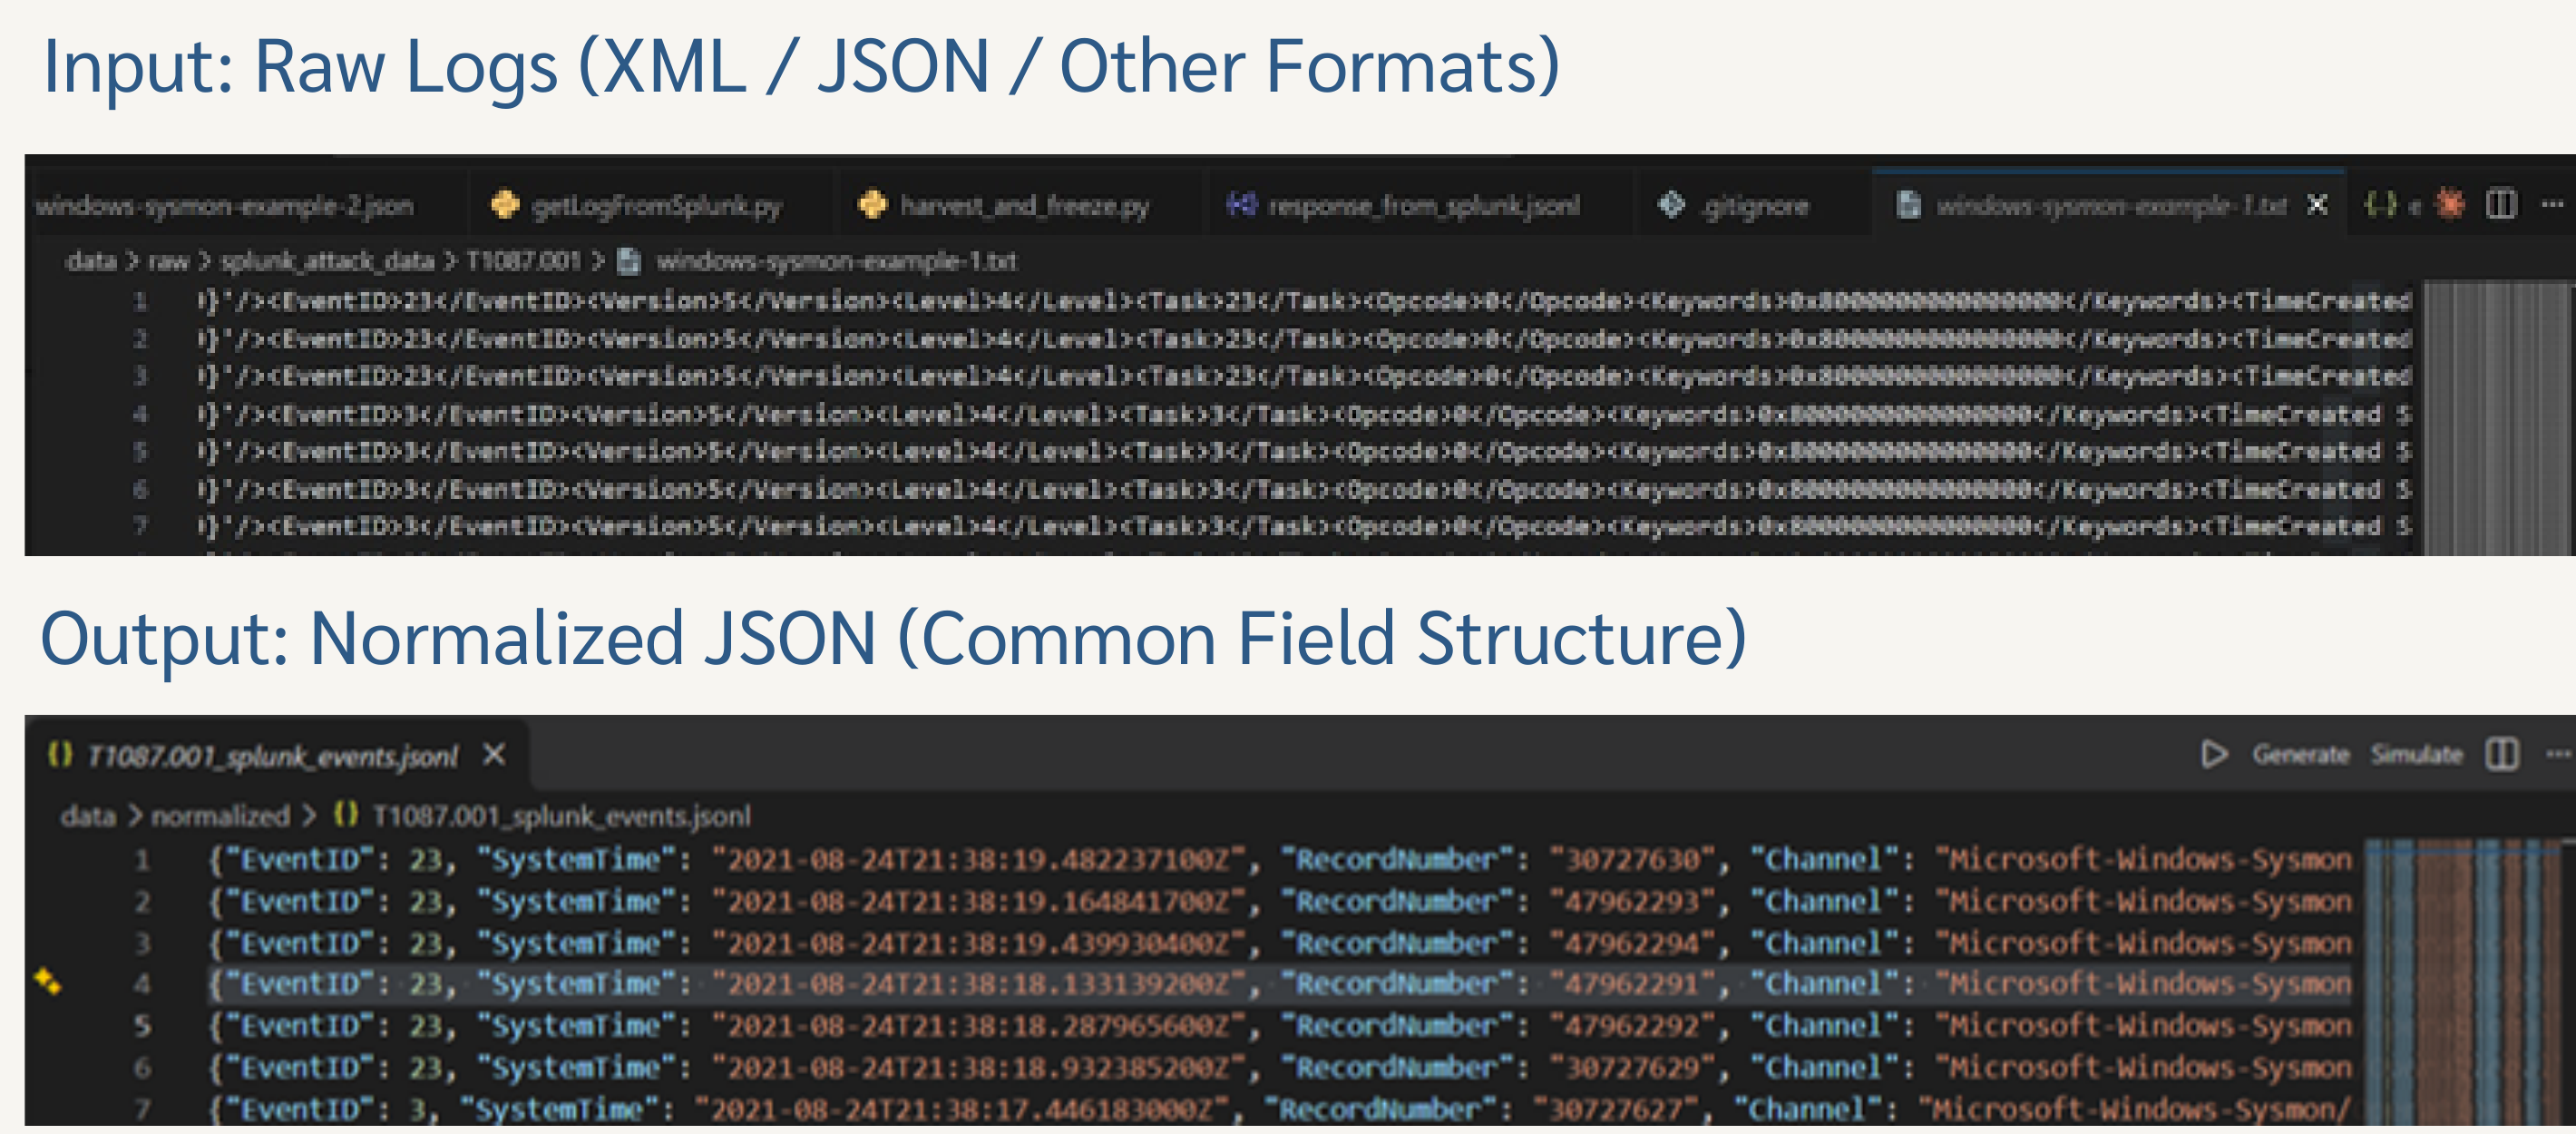
\includegraphics[width=\textwidth]{normalize_example.png}
  \caption{ตัวอย่าง Raw Logs (XML) และผลลัพธ์หลัง Normalize เป็น JSON}
  \label{fig:normalize}
\end{figure}

\subsection{ขั้นตอนที่ 3: Event Selection}
\label{sec:step-es}

Event Selection ตอบคำถามว่า \emph{``จะส่งเหตุการณ์ใดให้ LLM''}
ซึ่งเป็นขั้นตอนที่ยากที่สุดของ Pipeline เพราะต้องคัดเลือกให้ได้หลักฐานครบ แต่ไม่มี Noise มากเกินไป
โครงงานเปรียบเทียบวิธี Event Selection 5 วิธี โดย 4 วิธีแรกเป็นแนวทางพื้นฐาน
และวิธีที่ 5 (Top-$k$ Relevant Events) เป็นวิธีที่โครงงานนำเสนอ

\subsubsection{วิธี Event Selection ที่นำมาเปรียบเทียบ}
\label{sec:es-baselines}
แนวคิดของแต่ละวิธีแสดงในรูปที่~\ref{fig:es-methods} และข้อดีข้อเสียสรุปในตารางที่~\ref{tab:es-methods}

\begin{figure}[htbp]
  \centering
  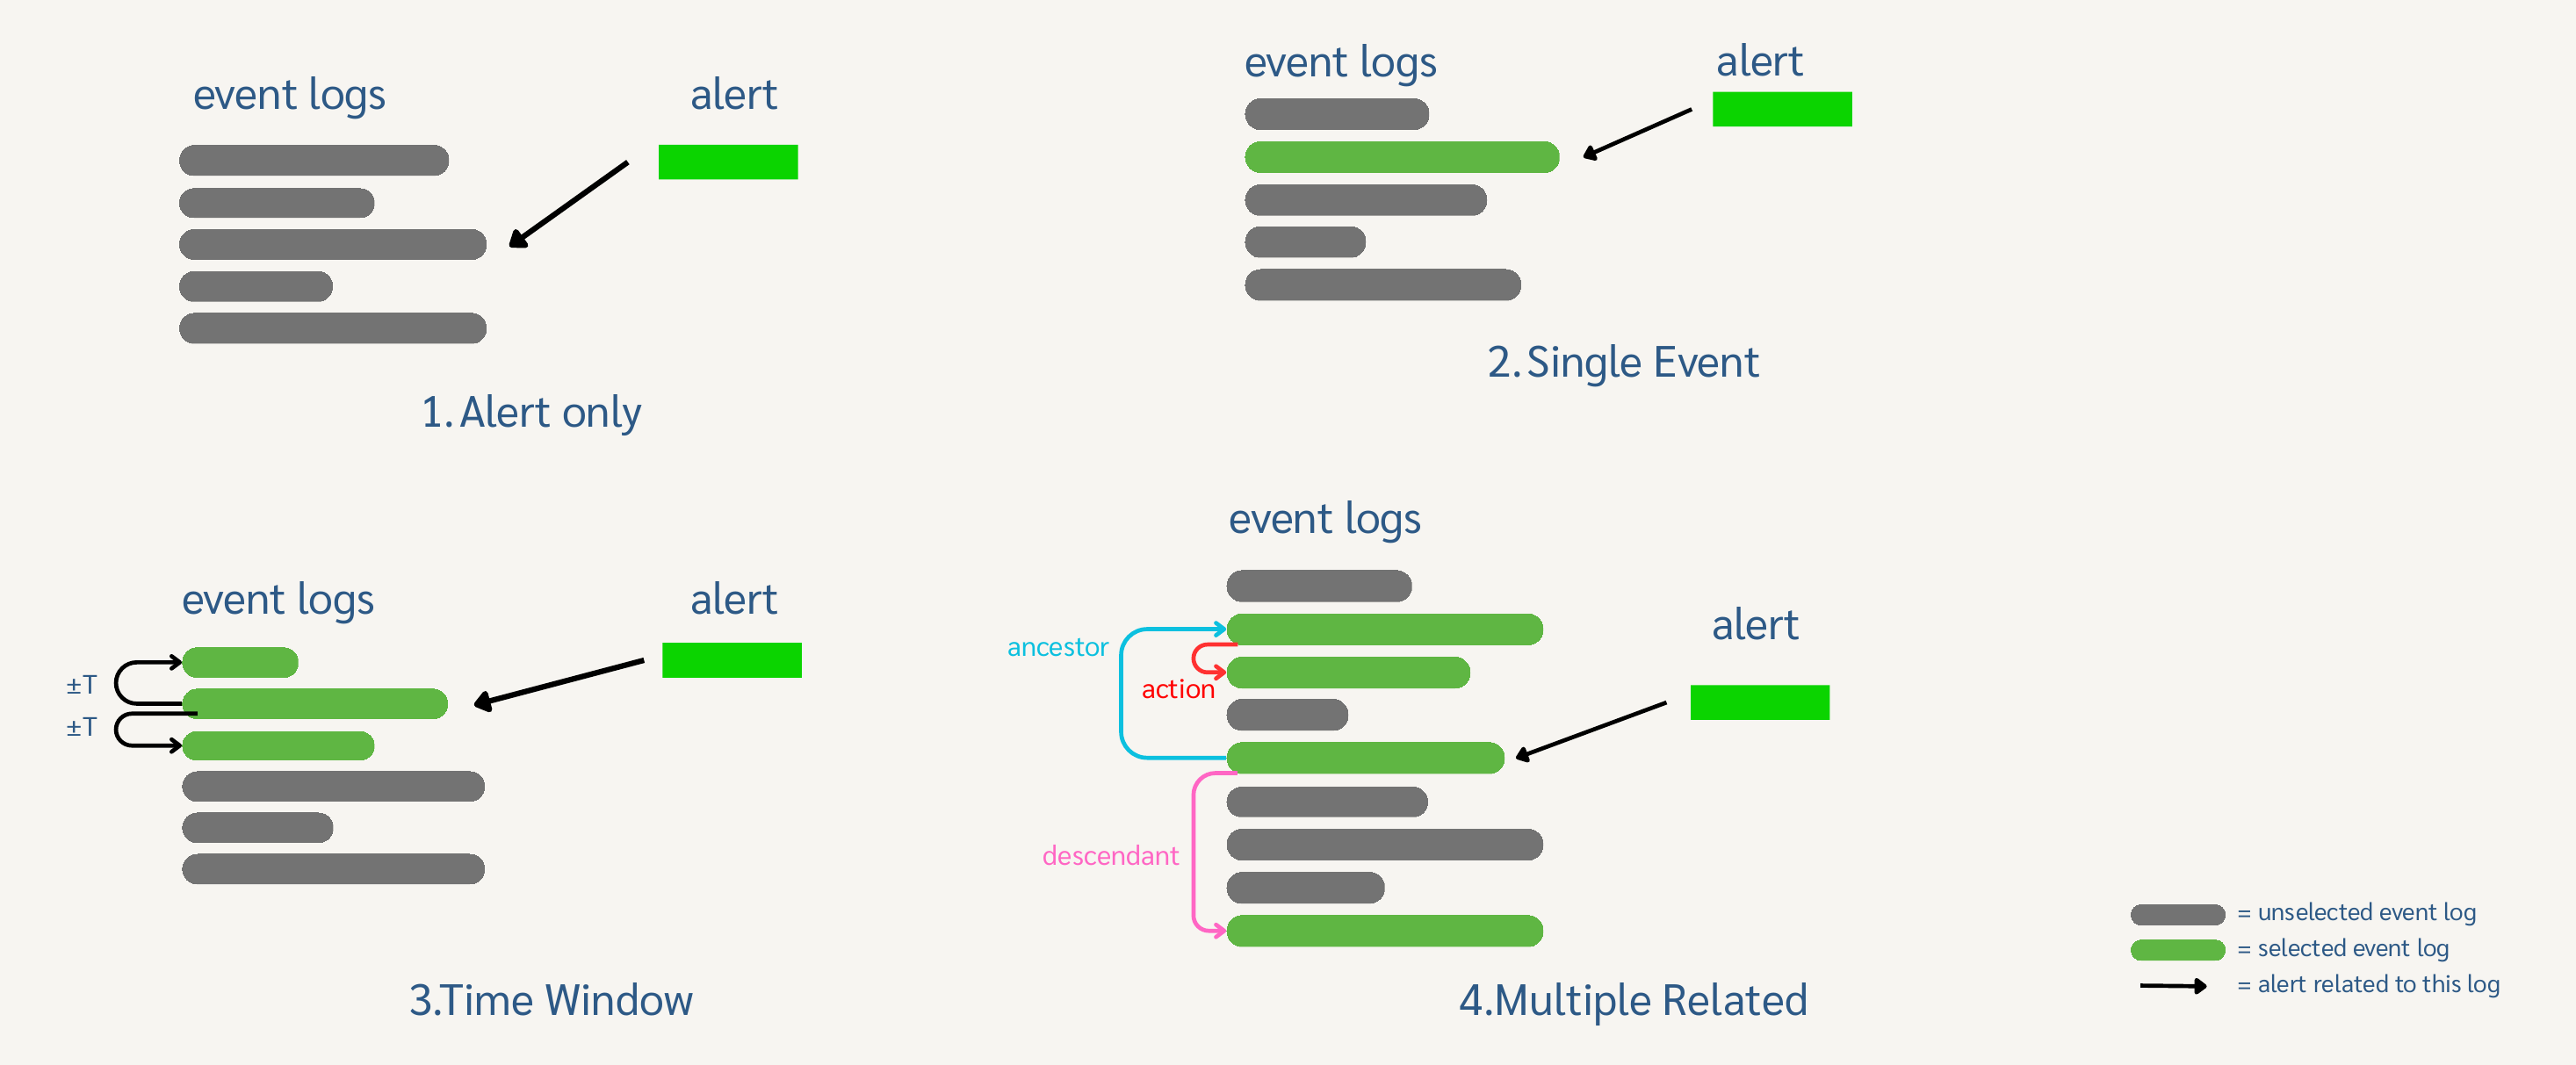
\includegraphics[width=\textwidth]{event_selection_methods.png}
  \caption{แนวคิดของวิธี Event Selection แบบที่ 1--4 (แถบสีเขียวคือ Event ที่ถูกเลือก)}
  \label{fig:es-methods}
\end{figure}

\begin{enumerate}
  \item \textbf{Alert Only} -- ใช้เฉพาะข้อมูลจาก Alert
  \item \textbf{Single Event} -- ดึงเฉพาะ Event เดียวที่ Alert ชี้
  \item \textbf{Time Window} -- ดึง Events ในช่วงเวลา $\pm T$ รอบ Alert
  \item \textbf{Multiple Related Events} -- ดึง Events ที่เชื่อมโยงกันจริงผ่านความสัมพันธ์ของ Process
        (ProcessGuid Lineage) ได้แก่ Ancestor, Descendant และ Events อื่นที่ ProcessGuid เดียวกัน
  \item \textbf{Top-$k$ Relevant Events} -- ให้คะแนนความเกี่ยวข้องกับทุก Event ในขอบเขตที่กำหนด
        แล้วเลือกเฉพาะ Events ที่มีคะแนนสูงสุดภายใต้งบประมาณ Token
\end{enumerate}

\begin{table}[htbp]
  \centering
  \caption{ข้อดีและข้อเสียของวิธี Event Selection แต่ละแบบ}
  \label{tab:es-methods}
  \begin{tabular}{|L{0.16\textwidth}|L{0.36\textwidth}|L{0.36\textwidth}|}
    \hline
    \textbf{วิธี} & \textbf{ข้อดี} & \textbf{ข้อเสีย} \\ \hline
    Alert Only &
      ประมวลผลเร็วที่สุด ไม่มี Overhead จากการ Query และใช้ได้แม้ไม่มี Raw Logs &
      ขาดหลักฐานเชิงลึก ไม่สามารถทำ Evidence Grounding ได้ LLM ได้แต่เชื่อตาม Alert \\ \hline
    Single Event &
      ได้รายละเอียดเต็มของ Event (CommandLine, GUID) และแยกผลของ ``รายละเอียด 1 Event'' ได้ชัด &
      ไม่เห็นว่า Event มาจากไหนหรือต่อไปทำอะไร พลาด Attack Chain ที่กระจายหลาย Event \\ \hline
    Time Window &
      Implement ง่าย (Range Query) ใช้ได้กับ Logs ทุกประเภท และจับ Events ที่เกิดพร้อมกันแต่ไม่เชื่อมกันทางโครงสร้างได้ &
      Noise สูงถ้า $T$ กว้าง พลาด Event ถ้า $T$ แคบ และไม่มีค่า $T$ ที่ถูกต้องสากล \\ \hline
    Multiple Related &
      สร้าง Attack Chain ได้ และตัด Events ที่เกิดพร้อมกันโดยบังเอิญออก &
      พึ่งพา Relationship Key สูง อาจพลาดพฤติกรรมที่ไม่เชื่อมทาง Process และเสี่ยง Over-traversal หากไม่จำกัดความลึก \\ \hline
    Top-$k$ Relevant &
      ควบคุมขนาด Context ได้ (Predictable Context Size) ยืดหยุ่น ปรับ $k$ ตามข้อจำกัด Token ได้ &
      ต้องออกแบบ Scoring Model ให้เป็น Generic และอ่อนไหวต่อค่า $k$ \\ \hline
  \end{tabular}
\end{table}

\FloatBarrier

\subsubsection{วิธีที่เสนอ: Top-$k$ Relevant Events}
\label{sec:topk}
จากตัวอย่าง T1087.001 เมื่อกำหนดให้ Alert ชี้ที่ Process \texttt{net.exe} (คำสั่ง \texttt{net users})
และใช้วิธี Multiple Related เพื่อดึง Process ที่เกี่ยวข้อง (ผู้ใช้ที่รัน, Parent และ Child Process)
พร้อม Events ที่ Process เหล่านั้นเป็นเจ้าของ จำนวน Events ลดลงจาก 11,090 เหลือ 177 Events
แต่จำนวน Events ที่ได้ยังขึ้นกับขนาดของ Process Tree และไม่มีการจัดลำดับความสำคัญ
วิธี Top-$k$ Relevant Events จึงต่อยอดจากแนวคิดนี้โดยให้คะแนนแต่ละ Event และคัดเลือกภายใต้งบประมาณ Token
แบ่งเป็น 4 ขั้นตอนย่อย ได้แก่ (i) Graph (ii) Traverse (iii) Score และ (iv) Budget ดังนี้

\topkstep{i. Graph -- สร้างกราฟความสัมพันธ์ของ Process}
สร้างกราฟความสัมพันธ์ระหว่าง Process และ Event โดยมีโหนดเป็น Process (ระบุด้วย ProcessGuid)
และเส้นเชื่อม 3 ประเภท ดังตารางที่~\ref{tab:graph-edges}
ทุก Event ถูกแนบกับโหนดของ Process เจ้าของ เมื่อการท่องกราฟไปถึงโหนดใดจะได้ Events ทั้งหมดของโหนดนั้น
ส่วน Process ที่ปรากฏเป็น Parent แต่ไม่มี EID 1 ในไฟล์ Log จะถูกตั้งเป็นโหนด Boundary ซึ่งเป็นจุดหยุดการท่องกราฟ

\begin{table}[ht]
  \centering
  \caption{ประเภทเส้นเชื่อมในกราฟความสัมพันธ์ของ Process}
  \label{tab:graph-edges}
  \small
  \begin{tabular}{|l|L{0.32\textwidth}|c|c|}
    \hline
    \textbf{เส้นเชื่อม} & \textbf{สร้างจาก} & \textbf{ใช้ท่องกราฟ} & \textbf{ระยะ (Cost)} \\ \hline
    Parent--Child & EID 1: \texttt{ParentProcessGuid} $\rightarrow$ \texttt{ProcessGuid} & ใช่ & 1 \\ \hline
    File--Exec & EID 11 ของ Process A สร้างไฟล์ X แล้ว EID 1 ของ Process B รันไฟล์ X & ใช่ & 1 \\ \hline
    Process Access & EID 10: Source $\rightarrow$ Target & ไม่ใช่ (แนบเป็นหลักฐาน) & 2 \\ \hline
  \end{tabular}
\end{table}

\noindent
Process Access (EID 10) ไม่ถูกใช้เป็นเส้นทางเดิน เนื่องจากมีสัดส่วนสูงใน Logs และส่วนใหญ่เป็นกิจกรรมปกติของระบบปฏิบัติการ
แต่จะถูกแนบเป็น Candidate ของโหนดที่เดินถึงแล้ว เพื่อให้ยังเห็นพฤติกรรมสำคัญ เช่น การเข้าถึงหน่วยความจำของ \texttt{lsass.exe}

\topkstep{ii. Traverse -- ท่องกราฟจากจุดที่ Alert ชี้}
\label{sec:traverse}
เริ่มจาก Process ที่ Alert ชี้ (Anchor) แล้วขยายไปยัง Parent และ Child Process
โดยเก็บเฉพาะบรรพบุรุษและลูกหลานโดยตรงที่อยู่ในระยะที่กำหนด
เพื่อให้ได้ Candidate Events ที่เกี่ยวข้องกับ Alert โดยไม่ลามไปทั้งระบบ ตามกฎดังนี้
\begin{enumerate}
  \item เดินตามเส้นเชื่อม Parent--Child และ File--Exec โดยหาเส้นทางที่มีระยะรวมน้อยที่สุด (Dijkstra)
  \item เดินทางเดียว คือขึ้นตรงหรือลงตรง ไม่เลี้ยวเข้ากิ่งข้างเคียง
  \item หยุดเมื่อครบจำนวน Hop สูงสุด หรือเจอ Boundary
        (Process ที่รู้ว่ามีอยู่ แต่ไม่มี EID 1 หรือบันทึกการเกิดในไฟล์ Log)
  \item ทุก Process ที่เดินถึง จะเก็บทุก Event ที่ Process นั้นเป็นเจ้าของ
\end{enumerate}
รูปที่~\ref{fig:traverse} แสดงส่วนหนึ่งของกราฟที่ได้จาก Sysmon Log ของ T1087.001
โดยเส้นทึบสีดำคือความสัมพันธ์ Parent--Child (EID 1) และเส้นประสีแดงคือ Process Access (EID 10)

\begin{figure}[ht]
  \centering
  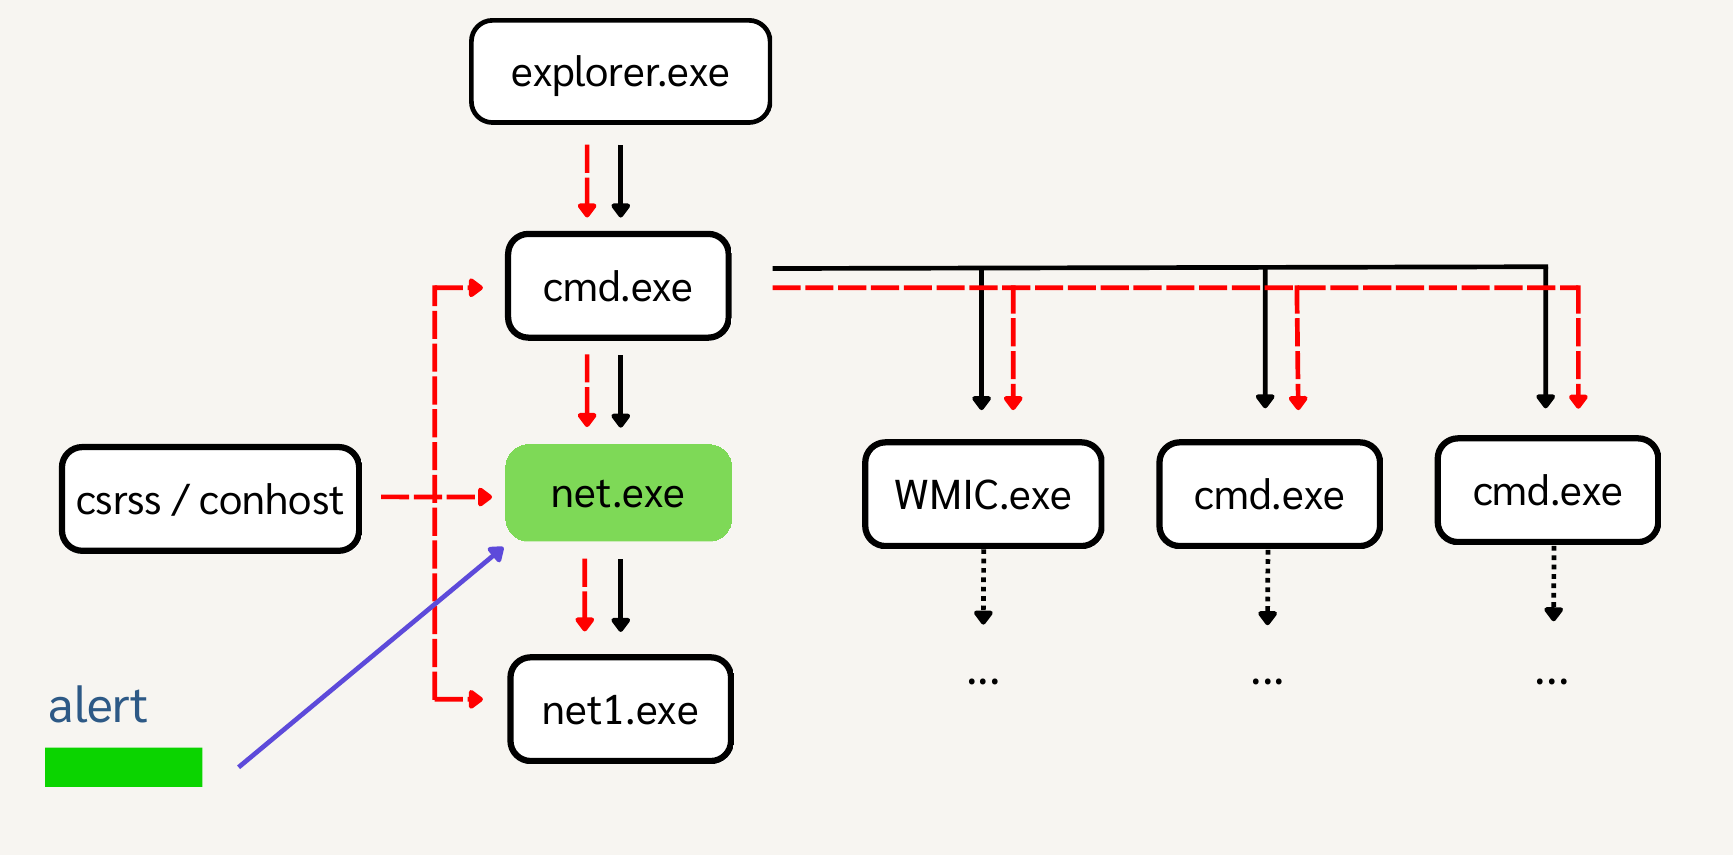
\includegraphics[width=0.85\textwidth]{traverse_graph.png}
  \caption{ส่วนหนึ่งของกราฟ Process จาก Sysmon Log ของ T1087.001 โดยมี \texttt{net.exe} เป็นจุดเริ่ม (Anchor)}
  \label{fig:traverse}
\end{figure}

การท่องกราฟขึ้นกับว่า Anchor มีสายความสัมพันธ์ของ Process (Lineage) หรือไม่ ซึ่งแบ่งได้เป็น 3 กรณี
\begin{enumerate}
  \item[A.] Anchor เป็น EID 1 และมี Lineage (เช่น \texttt{net.exe} ในกรณีนำร่อง) -- ท่องกราฟได้ตามปกติ
  \item[B.] Anchor ไม่ใช่ EID 1 แต่ Process เจ้าของมี EID 1 (เช่น Alert ชี้ EID 13 ของ \texttt{reg.exe})
        -- หาโหนดจาก ProcessGuid แล้วท่องกราฟต่อได้
  \item[C.] Process ของ Anchor ไม่มี EID 1 หรือทั้งไฟล์ไม่มี EID 1
        -- ไม่มีเส้น Parent--Child ให้เดินต่อ ได้เพียง Events ของ Process เดียวและ Events ที่แนบผ่าน EID 10
\end{enumerate}
สำหรับกรณี C จะกำหนดกติกาสำรองก่อนการปรับพารามิเตอร์ แนวทางที่พิจารณาคือ
เพิ่ม Events ในช่วงเวลา $\pm T$ บนเครื่องเดียวกันเป็น Candidate โดยกำหนดระยะเท่ากับจำนวน Hop สูงสุดบวกหนึ่ง
Events เหล่านี้จึงได้คะแนนต่ำกว่า Events ที่เชื่อมกันจริงเสมอ แต่ยังใช้เติมงบประมาณได้
ทุกกรณีทดสอบจะบันทึกว่าอยู่ในกรณี A, B หรือ C และรายงานผลแยกกลุ่ม
เพื่อแสดงว่าวิธี Top-$k$ ทำงานได้แย่ลงเพียงใดเมื่อไม่มี Lineage

\topkstep{iii. Score -- ให้คะแนนความเกี่ยวข้อง}
\textbf{หมายเหตุ:} สมการและค่าพารามิเตอร์ในขั้นนี้เป็นต้นแบบ (Prototype) และค่าเริ่มต้น
ที่ตั้งจากการวิเคราะห์กรณีนำร่อง T1087.001 เท่านั้น ยังไม่ใช่รูปแบบและค่าสุดท้าย
คณะผู้จัดทำจะปรับจูนทั้งรูปแบบของสมการและค่าพารามิเตอร์บน Development Set ภายหลัง
แล้วล็อกค่าก่อนนำไปใช้กับ Test Set

ประเมินและจัดลำดับความเกี่ยวข้องของแต่ละ Candidate Event $e$ ด้วยผลคูณของ 3 ปัจจัย ดังสมการ~\eqref{eq:score}

\begin{equation}\label{eq:score}
\mathrm{Score}(e) = \mathrm{Prox}(e) \times \mathrm{Type}(e) \times \mathrm{Time}(e)
\end{equation}
\begin{align}
\mathrm{Prox}(e) &= \gamma^{\,hop(e)} \\
\mathrm{Type}(e) &= w[\mathrm{EventID}] \\
\mathrm{Time}(e) &= e^{-|\Delta t|/\tau}
\end{align}

\noindent
โดยที่ $hop(e)$ คือจำนวนขั้นบนกราฟจากจุดที่ Alert ชี้ถึง Process เจ้าของ Event,
$\gamma$ คือสัดส่วนคะแนนที่เหลือเมื่อห่างออกไป 1 Hop,
$w[\mathrm{EventID}]$ คือน้ำหนักของ Event แต่ละชนิด (0--1) ที่บอกว่า Event ชนิดนั้นช่วยการวิเคราะห์ได้มากเพียงใด,
$\Delta t$ คือเวลาที่ห่างจาก Alert (วินาที) และ $\tau$ คือช่วงเวลาที่คะแนนลดลงเหลือประมาณ $1/e$ (ราว $1/3$)
ค่าเริ่มต้นของพารามิเตอร์แสดงในตารางที่~\ref{tab:score-param}
และตัวอย่างการคำนวณคะแนนแสดงในตารางที่~\ref{tab:score-example}

การรวมปัจจัยแบบผลคูณทำให้ Event ที่มีปัจจัยใดปัจจัยหนึ่งต่ำได้คะแนนต่ำโดยรวม
แนวทางการปรับจูนที่จะทดลองบน Development Set ได้แก่ การเปรียบเทียบกับรูปแบบอื่น
เช่น การรวมแบบผลรวมถ่วงน้ำหนัก (Weighted Sum) การตัดปัจจัยใดปัจจัยหนึ่งออกเพื่อดูผลของแต่ละปัจจัย (Ablation)
และวิธีนับระยะของ Events ที่แนบผ่าน Process Access
โดยใช้ Evidence Recall และความถูกต้องของ LLM บน Development Set เป็นเกณฑ์เลือก
ก่อนล็อกค่าและนำไปใช้กับ Test Set

\begin{table}[ht]
  \centering
  \caption{ค่าพารามิเตอร์เริ่มต้นของการให้คะแนน (จะปรับจูนบน Development Set ภายหลัง)}
  \label{tab:score-param}
  \begin{tabular}{|c|c|l|}
    \hline
    \textbf{พารามิเตอร์} & \textbf{ค่า} & \textbf{ความหมาย} \\ \hline
    $\gamma$ & 0.6 & Hop 0 = 1, Hop 1 = 0.6, Hop 2 = 0.36 \\ \hline
    $w[\text{EID 1}]$ & 1.0 & Process Creation มีข้อมูลคำสั่งครบ \\ \hline
    $w[\text{EID 10}]$ & 0.2 & Process Access ให้ข้อมูลประกอบ \\ \hline
    $\tau$ & 300 วินาที & ห่าง 300 วินาที คะแนนเวลาเหลือ 0.37 \\ \hline
  \end{tabular}
\end{table}

\begin{table}[ht]
  \centering
  \caption{ตัวอย่างการคำนวณคะแนนของ Candidate Events จาก T1087.001}
  \label{tab:score-example}
  \begin{tabular}{|l|c|c|c|c|c|c|}
    \hline
    \textbf{Event} & \textbf{Hop} & \textbf{$\Delta t$} & \textbf{Prox} & \textbf{Type} & \textbf{Time} & \textbf{Score} \\ \hline
    net1.exe (EID 1)         & 1 & 0.01 s & 0.6 & 1.0 & 1.00 & 0.60 \\ \hline
    cmd.exe (EID 1)          & 1 & 6.6 s  & 0.6 & 1.0 & 0.98 & 0.59 \\ \hline
    net $\rightarrow$ net1 (EID 10) & 0 & 0 s & 1.0 & 0.2 & 1.00 & 0.20 \\ \hline
    cmd $\rightarrow$ WMIC (EID 10) & 1 & 11 s & 0.6 & 0.2 & 0.97 & 0.12 \\ \hline
    cmd $\rightarrow$ cmd (EID 10)  & 1 & 74 s & 0.6 & 0.2 & 0.78 & 0.09 \\ \hline
  \end{tabular}

  \vspace{1mm}
  {\footnotesize หมายเหตุ: ค่า Hop ของ Events ชนิด EID 10 ในตารางนี้คำนวณด้วยวิธีนับ Hop แบบเดิม
  ซึ่งยังไม่ได้ใช้ระยะ (Cost) ตามตารางที่~\ref{tab:graph-edges}
  วิธีนับระยะของ EID 10 จะปรับในการทดลองขั้นต่อไป\par}
\end{table}

\topkstep{iv. Budget -- คัดเลือกภายใต้งบประมาณ Token}
เพื่อจำกัดจำนวน Token ให้พอดีกับ Context Window ของโมเดล และให้ LLM เห็นเฉพาะ Events ที่สำคัญที่สุดก่อน
ขั้นตอน Budget ทำงาน 3 ข้อ ดังนี้
\begin{enumerate}
  \item ใส่ Event ที่ Alert ชี้ (Anchor) เป็นอันดับแรก
  \item เรียง Events ที่เหลือตามคะแนนจากมากไปน้อย
  \item ใส่ทีละ Event พร้อมนับจำนวน Token สะสม หากเกินโควตา $B$ ให้หยุด
\end{enumerate}
ตัวอย่างเช่น หากกำหนดโควตา $B = 400$ Tokens และแต่ละ Event ใช้ประมาณ 100--130 Tokens
จะมีเพียงประมาณ 3 Events แรกเท่านั้นที่ถูกส่งต่อไปยังขั้นตอนถัดไป

\subsection{ขั้นตอนที่ 4: Representation}
\label{sec:step-rep}

Representation ตอบคำถามว่า \emph{``จะนำเสนอ Logs ที่คัดเลือกแล้วให้ LLM ในรูปแบบใดจึงเหมาะสมที่สุด''}
เนื่องจากข้อมูลชุดเดียวกันเขียนต่างรูปแบบกันจะได้จำนวน Token และความเข้าใจของ LLM ที่ต่างกัน
โครงงานเปรียบเทียบ 5 รูปแบบ (รูปที่~\ref{fig:representation} และตารางที่~\ref{tab:representation})
โดยพิจารณาตามลำดับความสำคัญ คือ (1) Accuracy ในการระบุเทคนิค และ (2) Token Efficiency

\begin{figure}[ht]
  \centering
  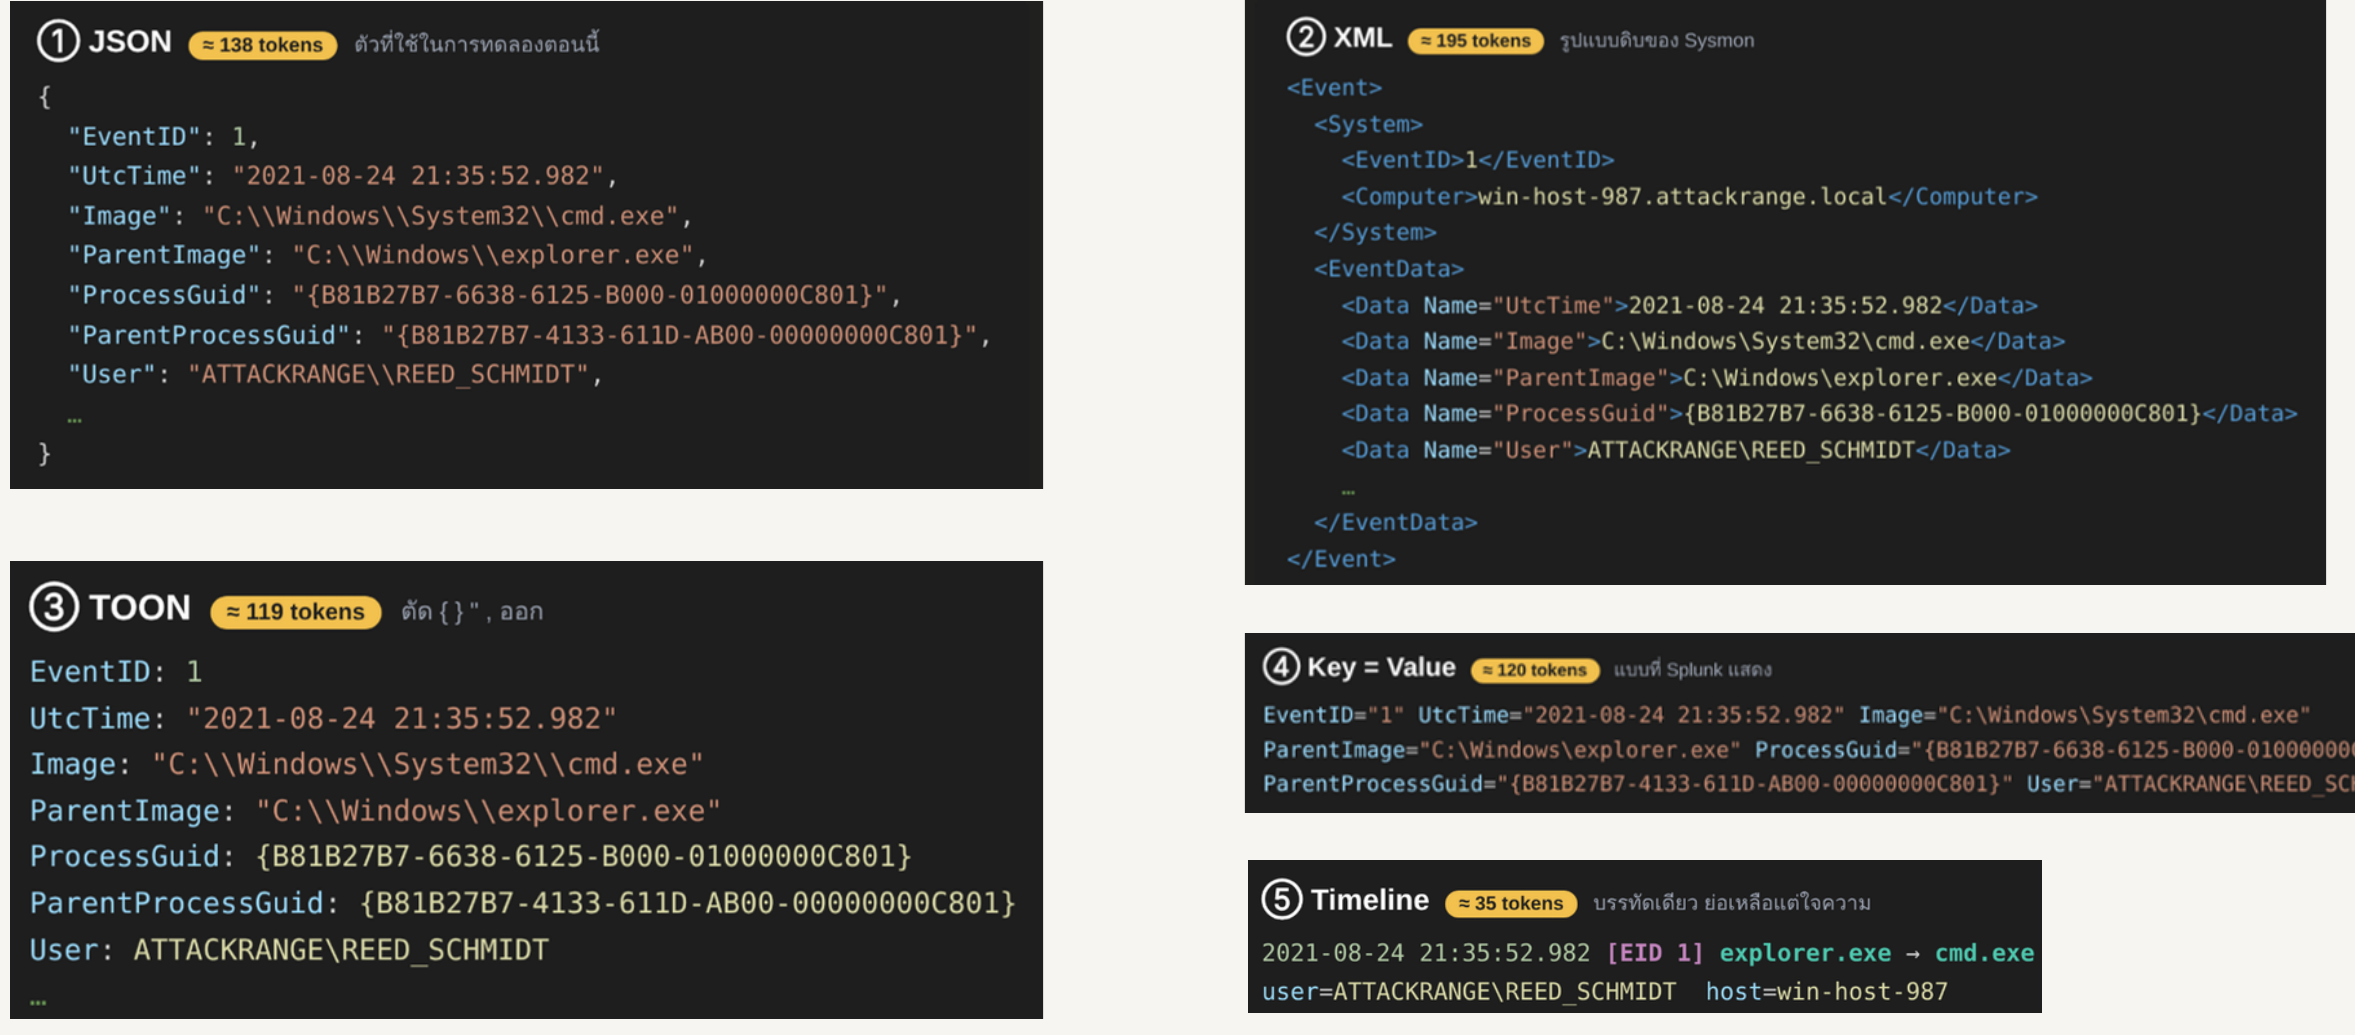
\includegraphics[width=\textwidth]{representation_formats.png}
  \caption{ตัวอย่าง Event เดียวกันในรูปแบบ JSON, XML, TOON, Key=Value และ Timeline}
  \label{fig:representation}
\end{figure}

\begin{table}[ht]
  \centering
  \caption{จำนวน Token โดยประมาณของ Event ตัวอย่าง (Sysmon EID 1) ในแต่ละรูปแบบ}
  \label{tab:representation}
  \begin{tabular}{|l|c|l|}
    \hline
    \textbf{รูปแบบ} & \textbf{Tokens (ประมาณ)} & \textbf{ลักษณะ} \\ \hline
    Timeline   & 35  & บรรทัดเดียว กระชับที่สุด แต่ข้อมูลบางส่วนหายไป \\ \hline
    TOON       & 119 & ตัด \{\} และ "" ออกจาก JSON \\ \hline
    Key=Value  & 120 & รูปแบบที่ Splunk แสดงผล \\ \hline
    JSON       & 138 & Output ของขั้นตอน Normalize (ใช้ในการทดลองปัจจุบัน) \\ \hline
    XML        & 195 & รูปแบบต้นฉบับของ Sysmon \\ \hline
  \end{tabular}
\end{table}

ในการทดลองปัจจุบันโครงงานเลือกใช้รูปแบบ JSON เนื่องจากได้มาโดยตรงจากขั้นตอนก่อนหน้า
ส่วนการเปรียบเทียบ Accuracy ระหว่างรูปแบบต่าง ๆ จะดำเนินการในการทดลอง E2 (หัวข้อ~\ref{sec:main-exp})

\subsection{ขั้นตอนที่ 5: Retrieval-Augmented Generation (RAG)}
\label{sec:step-rag}

RAG ทำหน้าที่เพิ่มบริบทให้ LLM โดยอ้างอิงองค์ความรู้จาก MITRE ATT\&CK
ฐานความรู้สร้างจากเอกสาร MITRE ATT\&CK Enterprise v19.2 (STIX ทางการ)
แปลงเป็น JSON และแบ่ง Chunk ตาม Technique และ Sub-technique
(1 Chunk ต่อ 1 Technique หรือ 1 Sub-technique) รวมทั้งหมด 697 Chunks (222 Techniques + 475 Sub-techniques)
ดังรูปที่~\ref{fig:rag-kb}
ข้อความของแต่ละ Chunk ประกอบด้วยชื่อ Tactics และคำอธิบาย (Description) โดยไม่ Embed รหัสเทคนิค
เหตุผลที่แบ่งถึงระดับ Sub-technique คือคำตอบที่ต้องการอยู่ในระดับ Sub-technique
และ Sub-technique ภายใต้ Technique เดียวกันมักต่างกันเพียงในคำอธิบาย
เช่น T1087.001 (\texttt{net user}) กับ T1087.002 (\texttt{net user /domain})
แต่ละ Chunk ถูกแปลงเป็นเวกเตอร์ด้วย \texttt{qwen3-embedding:0.6b} ผ่าน Ollama
ความยาวมัธยฐานของ Chunk ประมาณ 1,100 ตัวอักษร (ประมาณ 280 Tokens)

\begin{figure}[ht]
  \centering
  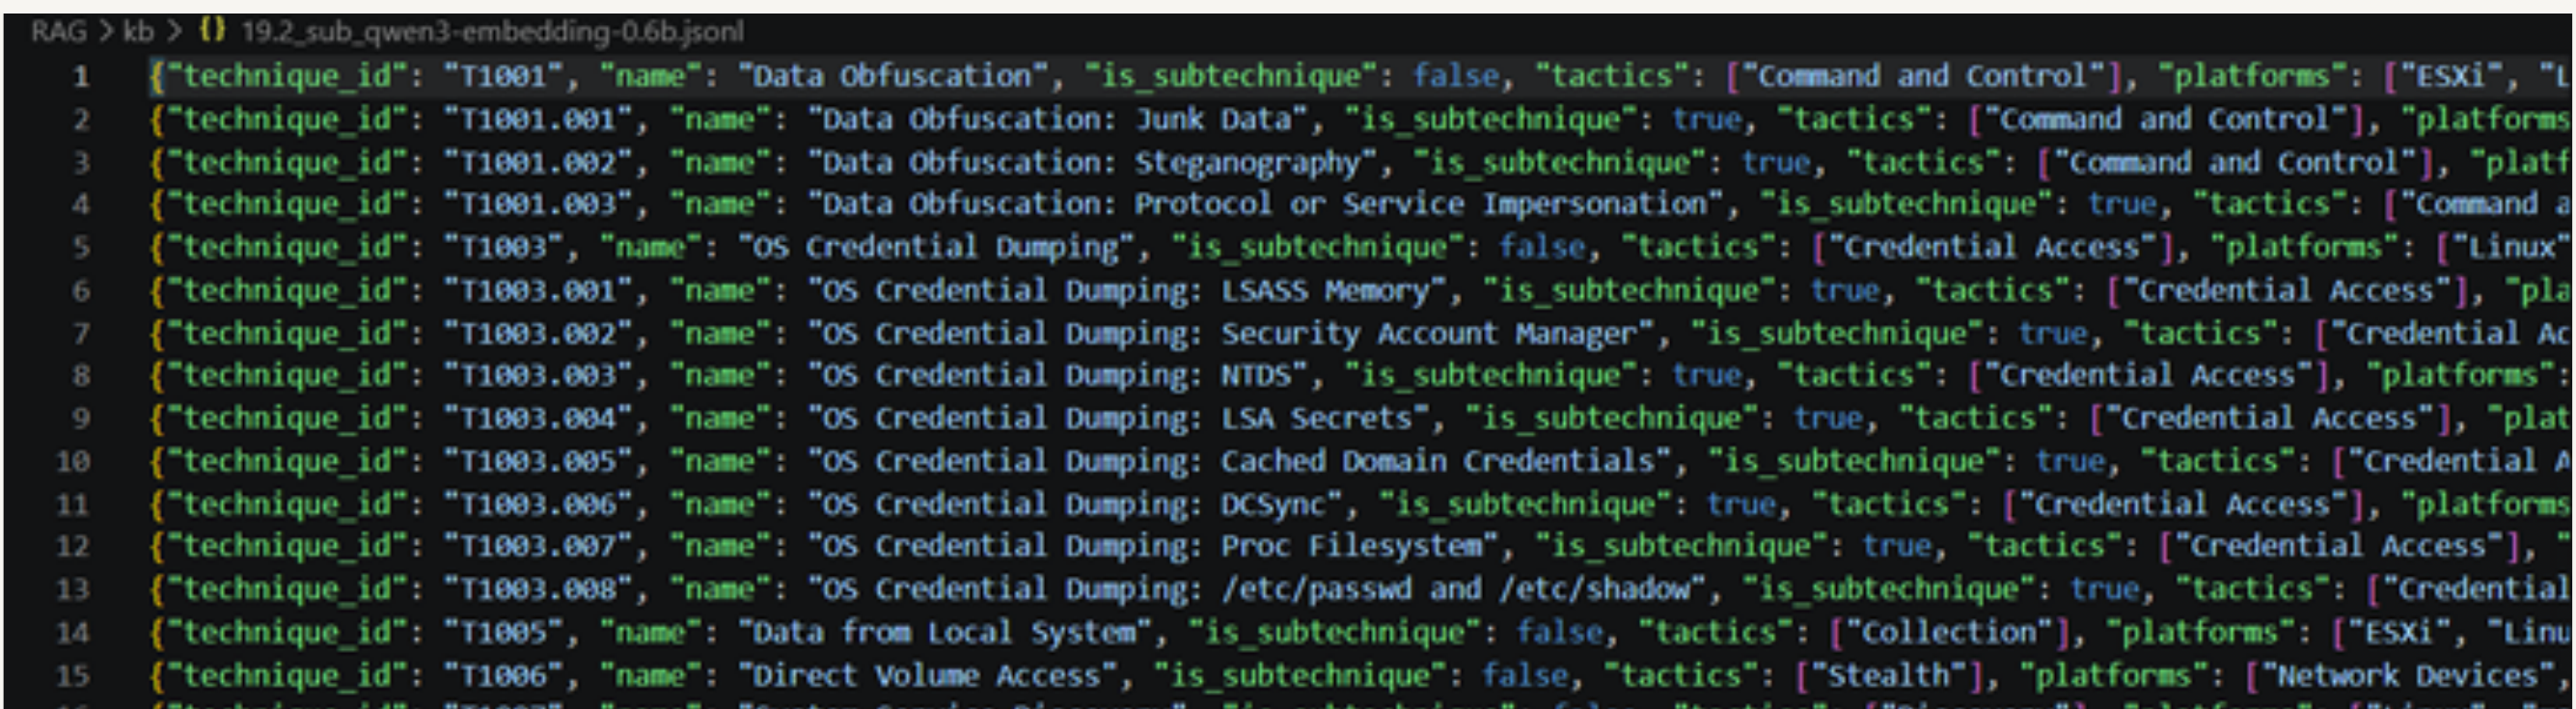
\includegraphics[width=\textwidth]{rag_kb_chunks.png}
  \caption{ตัวอย่างฐานความรู้ MITRE ATT\&CK v19.2 ที่แบ่ง Chunk ตาม Technique และ Sub-technique}
  \label{fig:rag-kb}
\end{figure}

Query ที่ใช้ค้นหาในฐานความรู้มีได้ 2 แบบ คือ
(1) ใช้ Representation Log (JSON) โดยตรง และ
(2) ให้ LLM แปลง Representation Log เป็นคำอธิบายพฤติกรรมภาษาอังกฤษ (Log Summary) ก่อน
โดยห้ามใช้ชื่อหรือรหัสเทคนิค ผลลัพธ์ของ RAG คือรายการ Top-$k$ Techniques ที่ใช้เป็น Context ให้ LLM

\subsection{ขั้นตอนที่ 6: LLM Analysis และ Output}
\label{sec:step-llm}

LLM ที่ใช้คือ Qwen3.5:9B ทำงานภายในเครื่องผ่าน Ollama ร่วมกับ Hermes เป็น Harness
LLM รับ Context จาก RAG และ Representation Log แล้วระบุเทคนิคการโจมตี
Prompt ถูกออกแบบให้ LLM ทำงานเป็นลำดับ ได้แก่
อ่าน Event ที่ Alert ชี้ก่อน $\rightarrow$ พิจารณาว่าคำสั่งทำอะไร $\rightarrow$ ระบุ Technique
$\rightarrow$ ระบุ Sub-technique ที่ตรงกับรูปแบบคำสั่ง $\rightarrow$ ระบุทางเลือกที่ใกล้เคียงและเหตุผลที่ไม่ใช่
และตอบในรูปแบบ JSON ที่มีโครงสร้างกำหนด (เช่น พฤติกรรมที่สังเกตได้ ทางเลือกที่พิจารณา รหัสเทคนิค และความมั่นใจ)
สำหรับกรณีใช้ RAG จะระบุใน Prompt ว่ารายการ Candidate เป็นเพียงคำใบ้ และคำตอบที่ถูกอาจไม่อยู่ในรายการ
การตั้งค่าในการทดลอง ได้แก่ ปิดโหมด Thinking, Temperature = 0 และ Context Window 16,384 Tokens

เพื่อป้องกันการรั่วไหลของเฉลย ระบบจะตรวจสอบว่า Prompt และ Query ไม่มีรหัสเทคนิค
(รูปแบบ \texttt{T\#\#\#\#}) หรือรหัส Case ที่บอกคำตอบ ก่อนส่งให้ LLM
ผลลัพธ์สุดท้ายคือ Investigation Report ที่ระบุเทคนิค ATT\&CK หลักฐาน (Event ที่อ้างอิง) และเหตุผลประกอบ

\section{ต้นแบบ Web Dashboard}
\label{sec:dashboard}

ผลการวิเคราะห์ถูกนำเสนอให้ SOC Analyst ผ่าน Web Dashboard
ซึ่งออกแบบให้รับข้อมูลได้ 2 แบบ คือ อัปโหลดไฟล์ Logs ด้วยตนเอง (Manual Investigation) ซึ่งเป็นแบบที่ใช้ในระยะนี้
และรับ Alert จาก SIEM อัตโนมัติ ซึ่งจะพัฒนาในระยะถัดไป
หน้า Inbox (รูปที่~\ref{fig:dashboard}) แสดงรายการการสืบสวนทั้งหมด พร้อมแหล่งที่มา ความรุนแรง เวลา
ชื่อ Alert และ Host สถานะการประมวลผลของ LLM (Pending, Processing, Analyzed, Failed)
ผลลัพธ์ (เทคนิคที่ระบุได้) และผู้รับผิดชอบ
นอกจากนี้ยังมีเมนูสำหรับผู้ดูแลระบบ เช่น การเชื่อมต่อ SIEM การตั้งค่า Pipeline
และการปรับปรุงข้อมูล/ฐานความรู้ ซึ่งกำหนดให้ผู้ดูแลระบบเป็นผู้สั่งปรับปรุงเท่านั้น

\begin{figure}[htbp]
  \centering
  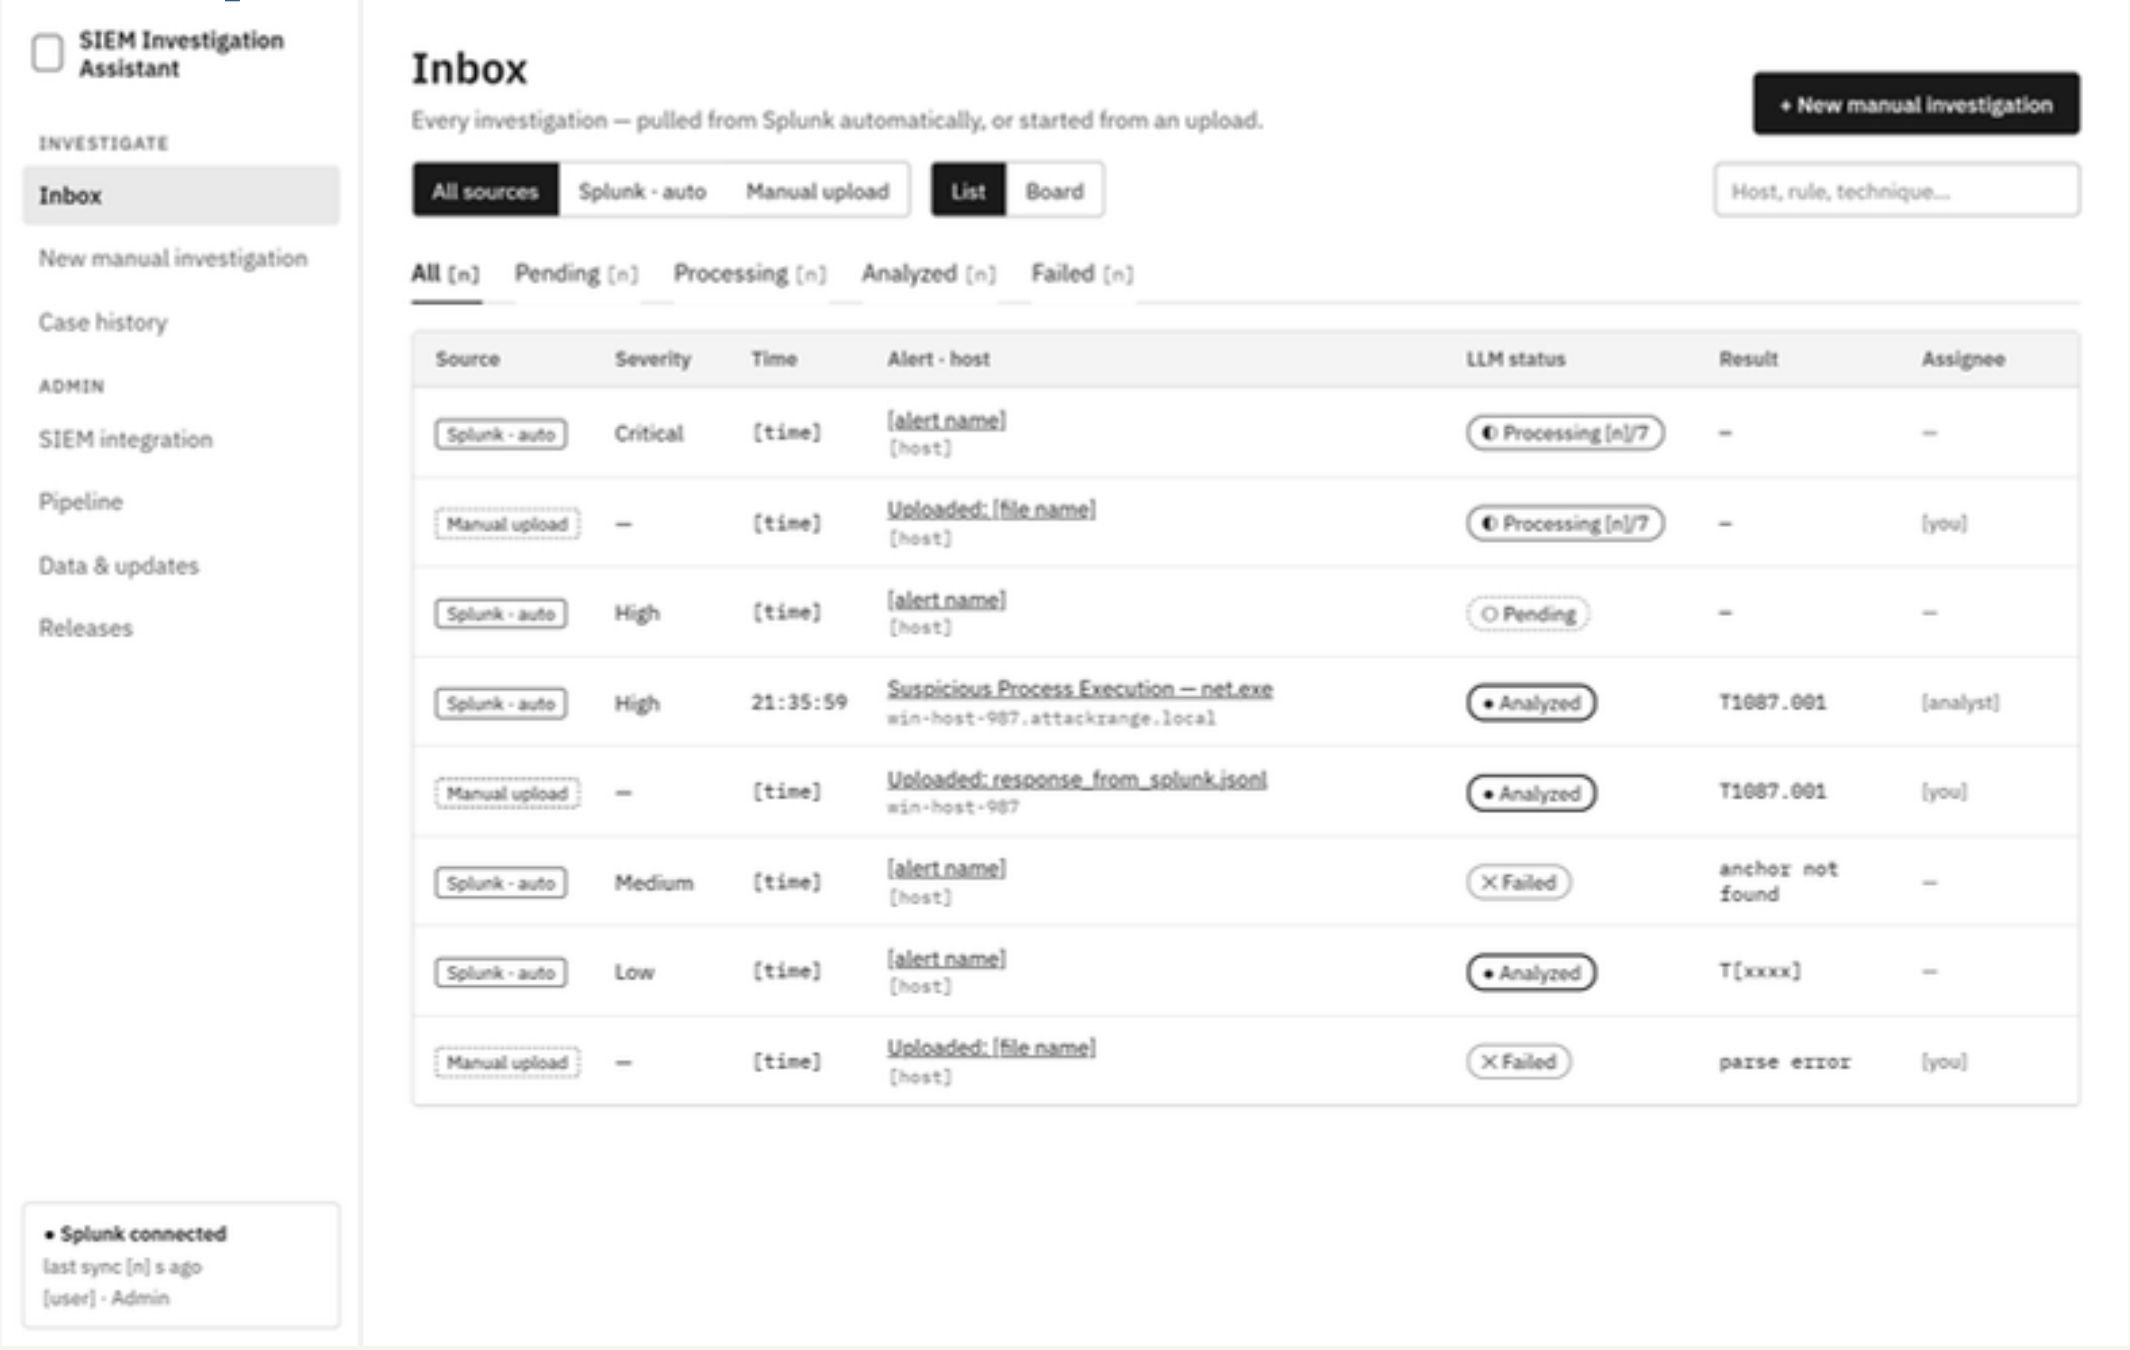
\includegraphics[width=\textwidth]{dashboard_prototype.png}
  \caption{ต้นแบบหน้า Inbox ของ Web Dashboard}
  \label{fig:dashboard}
\end{figure}
